This section describes the purpose, use and intended user audience for the Fiducial Career Display.
The purpose of this  project is to build a top flat surface table with that  provides user
interface with needed information. The system consists of fiducial markers which will be placed on
top of the surface of the table and will be able to move around the surface.

\subsection{Purpose and Use}
This product is meant to replace the iPad career wall in the Air Force Performance Lab.
Each fiducial markers will display a career available in the Air Force.
When the marker is placed on the table, an interface will appear to allow the user to page through different details about that career.
Any user can walk up and pick up a maker and start interacting to explore the career description.
Their objective is to change people\'s perceptions about what the Air Force does and inspire them to learn more while
generating qualified leads.

\subsection{Intended Audience}
The intended audiences of the product include:
\begin{itemize}
\item The recruitment officer, who can show the information for intended audience
\item The visitor, normal people who interested in the Air Force careers can look into it and find the materials they need
\end{itemize}


Note: This product was designed specifically for the Air Force Performance Lab, but it can be repurposed to other commercial uses such as museums, trade shows and so on...
\begin{figure}[h!]
	\centering
   	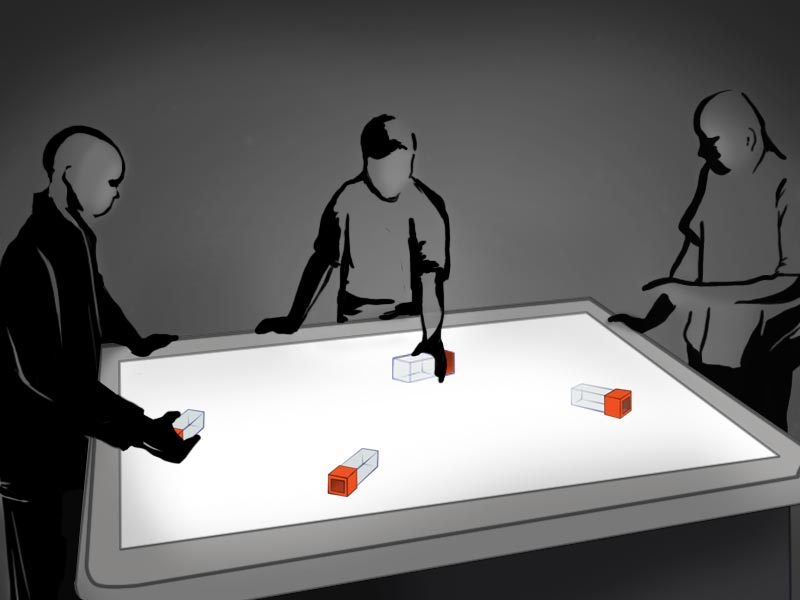
\includegraphics[width=0.8\textwidth]{images/Concept_Sketches_03}
    \caption{Table conceptual drawing \cite{concept1}}
\end{figure}
